\setcounter{section}{1} % This causes the next section to be Appendix B


\section*{Examples II: Kinetics, Constitutive Laws, and Viscoelasticity I}
\label{PS2}
\textcolor{red}{(Rev note: v2)}


This set of example problems is due on October 3, 2025. 
As before, I request that you type up your responses in \LaTeX~ rather than write them out by hand. 

\medskip
\subsection*{2--1. \textbf{Balance of mass} [4 pts].} 
A large piece of polydimethylsiloxane (PDMS) of uniform density $\rho(\bm{x},t)$ has a central spherical bubble of time-evolving radius $R(t)$, initial radius $R_0$, and wall velocity of $\dot{R}$. 
The hole is subject to a uniform surface traction in the $\bm{e}^{(r)} \equiv \bm{e}_{\bm{r}}$ direction from an axisymmetric pressure, and maintains spherical symmetry over time. 

\medskip
The position of a point in the material can be written as $\bm{x} = r(R,t) \bm{e}_{\bm{r}}$ with reference position $\bm{X} = r_0(R_0)$, while the velocity of that point can be written as $\bm{v}(r,t) = v_r \bm{e}_{\bm{r}}$.

\medskip
Using the conservation of mass equation, show that the material must satisfy
%\begin{equation}
%\rho_{,t} + (\rho v_i)_{,i} = 0,
%\end{equation}
\begin{equation*}
\rho_{,t}+ \rho_{,r} v_r + \frac{\textcolor{red}{2}\rho}{r} (v_r + r v_{r,r}) = 0,
\end{equation*}
and hence, show that an assumption of incompressibility for PDMS results in 
\begin{equation*}
v_r(r,t) = \frac{R^2 \dot{R}}{r^2}.
\end{equation*}

\subsection*{2--1}
With banlance of mass law in spherical coordiantes, we have:
$\frac{\partial\rho}{\partial t}+\frac1{r^2} \frac{\partial(\rho r^2 v_r)}{\partial r} =0$ (Eliminate the components of $v_{\theta}$ and $v_{\phi}$) \\
Thus, we would have 
\begin{align*}
    \rho_{,t}+\frac1{r^2}[\rho_{,r}r^2 v_r+2\rho r v_r +\rho r^2 v_{r,r}]&=0 \\
    \rho_{,t}+ \rho_{,r} v_r + \frac{\rho}{r} (2v_r + r v_{r,r}) &= 0 \\
\end{align*}
For the assumption of incompressibility, we assume that $\rho$ is constant, thus we have 
\begin{align*}
    2v_r + rv_{r,r}&=0 \\
    \frac{2\partial r}{r} &= - \frac{\partial v_r}{v_r} \\
    2 \ln{r}&= -\ln{v_r} + C 
\end{align*}
For the boundary condition, we have: when $r=R(t),\ v_r = \dot{R}$.\\
Thus,
\begin{align*}
    2 \ln{R} &= -\ln{\dot{R}} +C\\
    C&= \ln{R^2 \dot{R}}
\end{align*}
Hence,
\begin{align*}
    2 \ln{r}&= -\ln{v_r} +\ln{R^2 \dot{R}} \\
    \ln{v_r} &= \ln{\frac{R^2 \dot{R}}{r^2}} \\
    v_r(r,t) &= \frac{R^2 \dot{R}}{r^2}
\end{align*}

\medskip
\subsection*{2--2. \textbf{Balance of momenta} [4 pts].} A spherical hydrogel body $\mathcal{B}$ with a linear density gradient is currently submerged in water as depicted in the figure. 
The sphere has coordinates $\bm{x}$ in a region $\Omega$ with position-dependent density $\rho(\bm{x})$. 

\begin{figure}[H]
\vspace{-2em}
\centering
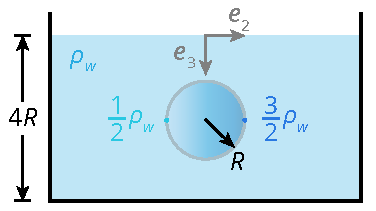
\includegraphics[width=3in]{instr-figures/PS2-Q1.pdf}
\caption{\small{Hydrogel sphere with a linear density gradient submerged in water. The water has a density $\rho_w$, while the sphere has a density at its leftmost point of $\rho_w/2$ and at its rightmost point of $3\rho_w/2$.}}
\end{figure}

\vspace{-1em}
The surface traction $\bm{t}(\bm{x},\hat{\bm{n}})$ acting on $\mathcal{B}$ is given by 
\begin{equation*}
\bm{t}(\bm{x},\hat{\bm{n}}) = -\rho_w g x_3 \hat{\bm{n}},
\end{equation*}
where $\hat{\bm{n}}$ is the outer unit normal to the surface $\partial \Omega_t$ and $\rho_w$ is the (constant) density of water and $g$ is the acceleration due to gravity. 

\medskip
(a) Determine the net force and moment acting on $\mathcal{B}$ via volume integrals.

\medskip
(b) Under what \textit{two} conditions is $\mathcal{B}$ in static equilibrium?

\subsection*{2--2}
The force of the surface traction from water is
\begin{equation*}
    \bm{F_w} = \int\limits_{\partial \mathcal{B}} -\rho_w g x_3 \hat{\bm{n}}dA =-\rho_w g \int \limits_\mathcal{B}\nabla{x_3}dV =-\rho_w g V\bm{e_3} = -4/3\pi p_wgR^3 \bm{e_3}
\end{equation*} \\
The gravitational force is
\begin{align*}
    \bm{F_g}& = \int \limits_{\mathcal{B}}\rho(\bm{x})\bm{g}dV \\
    &=\bm{g} 
    \int^{R}_{-R}\pi (R^2-x^2_2)(\frac{\rho_w}2 +\frac{\rho_w}{2R} x_2)dx_2  \\
    &= \frac23 \pi \rho_w R^3g \bm{e_3}
\end{align*}
Thus, the net force is $\bm{F_{net}} = \bm{F_w} +\bm{F_g} = -\frac23 \pi \rho_w R^3g \bm{e_3}$ \\

Let's say the center of the sphere is $\bm{x_c}=(x_c,y_c,z_c)$, each point is distanced from it with a vecotr $\bm{r}=(x_1,x_2,x_3)$. Thus, the moment from water traction is 
\begin{align*}
     \bm{J_w} &= \int\limits_{\partial \mathcal{B}} -\rho_w g  \bm{r} \times (z_c+x_3) \hat{\bm{n}}dA \\
     &=  -\rho_w g\int\limits_{\partial \mathcal{B}}(z_c+x_3)(\bm{r}\times\hat{\bm{n}})dA  \\
     &= 0
\end{align*}
$\bm{r}\times\hat{\bm{n}}=0$ since $\hat{\bm{n}}=\frac{\bm{r}}{|\bm{r}|}$ and $\bm{r}\times\bm{r}=0$ \\
For the angular momentum from gravity,
\begin{align*}
    \bm{J_g}&= 
    \int\limits_{\mathcal{B}} \bm{r} \times (\frac{\rho_w}2 +\frac{\rho_w}{2R} x_2)g\hat{\bm{e_3}}dV  \\
    &=-\rho_w g \int\limits_{\mathcal{B}}(\frac12 +\frac{x_2}{2R})( \bm{r} \times \hat{\bm{e_3}})dV\\
    &=-\rho_w g \int\limits_{\mathcal{B}}(\frac12 +\frac{x_2}{2R})
    \begin{pmatrix}
        -x_2 \\x_1 \\0
    \end{pmatrix}dV
\end{align*} \\
For the x component, the integral simplifies to $\rho_w g \int\limits_{\mathcal{B}}\frac{x_2^2}{2R}dV$ since the other term is odd function across V. Then the integral goes to
\begin{align*}
    \rho_w g \int\limits_{\mathcal{B}}\frac{x_2^2}{2R}dV
    &=\rho_w g \int^{R}_{-R}\frac{x_2^2}{2R}\pi(R^2-x_2^2)dx_2\\
    &=\frac2{15}\pi\rho_w g R^4 \\
    \end{align*}
As for the y component, since it's also odd function across V, thus it's 0. \\
Therefore, the moment of fravity force is $(\frac2{15}\pi\rho_w g R^4,0,0)$. The net moment is $(\frac2{15}\pi\rho_w g R^4,0,0)$.

\medskip
(b)
1) The buoyancy force should balance the gravity, so the only volume that the ${\mathcal{B}}$ can be submerged is $ \frac{\bm{F_g}}{\rho_{\omega}g\bm{e_3}}= \frac23 \pi R^3$, only $\frac12$ of the sphere can be submerged.\\
2) The angular momentum should be zero. So the gradient of the density should on the $\hat{\bm{e_3}}$ direction, so that in the integral $\int\limits_{\mathcal{B}}(\frac12 +\frac{x_3}{2R})
    \begin{pmatrix}
        -x_2 \\x_1 \\0
    \end{pmatrix}dV$ equals 0.


\bigskip
\subsection*{2--3. \textbf{Viscoelastic data} [4 pts].} 
Stress relaxation isochrones for a compliant viscoelastic material are shown in the figure below.  

\begin{figure}[H]
\vspace{-1em}
\centering
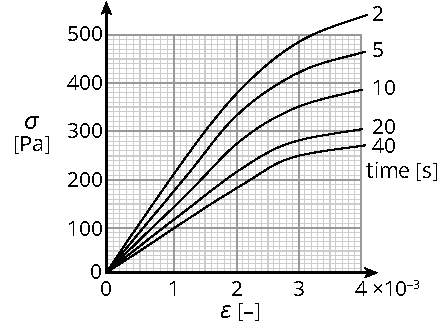
\includegraphics[scale = 1.5]{instr-figures/PS2-Q3.pdf}
\caption{\small{Stress (Pa) vs. strain ($-$) for a soft viscoelastic material.}}
\end{figure}

\vspace{-1em}
(a) Are these isochrones from a material which we can describe with linear viscoelasticity? If not, why not, and if so, under what approximate regimes would this assumption be valid? 

\medskip
(b) Estimate the creep relaxation function $J_c$ for stress values of 100 and 250 \textcolor{red}{Pa}. Isochrones are shown at times of 2, 5, 10, 20, and 40 seconds.   
% This is a placeholder for the example problems from the second problem set. 
% You'll replace this file with the one I supply on canvas.

\subsection*{2--3}
(a) Yes it can be called a material with linear viscoelasticity. when the strain is from 0 to $2 \times 10^{-3}$, they are in linear viscoelasticiy regime. \\
\\
(b) When $\sigma = 100$ Pa, the strain is about 0.43, 0.52, 0.66,0.81,1.0  at 2, 5, 10, 20, 40 s  gives a Jc of 2.867, 3.467, 4.400, 5.400, 6.667 $\times10^{-6} Pa^{-1}$

\bigskip
\subsection*{2--4. \textbf{Impulsive stresses} [4 pts].}

(a) Say that instead of a step load, we apply $\sigma(t) = A \delta(t)$ to an unknown linear viscoelastic material. 
Determine the strain history $\epsilon(t)$, first as a general function of the creep relaxation function $J_c(t)$, and then for a Kelvin-Voigt solid. 

(b) Now, consider a rapid load followed by a rapid reverse load by applying a doublet function of stress, i.e. $\sigma(t) = B \psi(t)$. 
What is the strain function $\epsilon(t)$ in terms of $J_c(t)$ and for a Kelvin-Voigt material now? 

\subsection*{2--4}
(a) 
For a general function, 
\begin{equation*}
    \epsilon(t) = \int^t_0 J_c(t-\tau)\frac{d(A\delta(\tau))}{d\tau}d\tau = \int^t_0 J_c(t-\tau) A \psi(\tau)d\tau
\end{equation*} \\
For a K-V model, we have
\begin{equation*}
    \epsilon(t) = \frac{A\delta(t=0^-)}{E}(1-\exp(-Et/\eta)) + \frac1E \int^t_{0^-}[1-\exp(-E(t-\tau)/\eta)]A\psi(\tau)d\tau
\end{equation*} \\

(b)
For a general function, 
\begin{equation*}
    \epsilon(t) = \int^t_0 J_c(t-\tau)\frac{d(B\psi(\tau))}{d\tau}d\tau = \int^t_0 J_c(t-\tau) B \frac{\partial \delta(\tau)^2}{\partial^2 \tau}d\tau
\end{equation*} \\
For a K-V model, we have
\begin{equation*}
    \epsilon(t) = \frac{B\psi(t=0^-)}{E}(1-\exp(-Et/\eta)) + \frac1E \int^t_{0^-}[1-\exp(-E(t-\tau)/\eta)]B \frac{\partial \delta(\tau)^2}{\partial^2 \tau}d\tau
\end{equation*}

\bigskip
\subsection*{2--5. \textbf{Two-element models} [8 pts].}

Dynamic mechanical analysis (DMA) is a common technique for characterizing viscoelasticity. 
DMA conventionally involves application of a sinusoidal displacement to the top surface of a sample at a controllable temperature. 
Often, the user puts the sample into initial compression, and follows with the sinusoidal profile. 
A cylindrical sample of height $h$ and diameter $d$ is placed between two plates.
The DMA then quickly puts the sample into compression by moving its top plate downward by a displacement $d$, and then oscillates sinusoidally between positions $0$ and $2d$ at a frequency $\omega$.

\medskip
(a) Using the constitutive law for a Kelvin-Voigt material, determine the stress $\sigma(t)$ exerted by the platens to cause the applied strain. 

\medskip
(b) The resulting stress lags behind the strain by an phase $\delta$, as in $\sin(\omega t + \delta)$. 
Commonly this is reported as the ``tangent loss", or $\tan\delta$, for a material. 
What is the value of $\tan\delta$ for this particular Kelvin-Voigt model?

\medskip
(c) Say instead of prescribing the strain $\epsilon(t)$, we instead prescribed the stress, $\sigma(t) = - \sigma_0 - \sigma_0 \sin(\omega t)$. 
Determine the strain $\epsilon(t)$ for this prescribed stress.

\medskip
(d) Prove that the tangent loss function $\tan\delta$ is identical between the two loading methods.

\subsection*{2--5}
(a) $\epsilon(t)=d+d\sin(\omega t)$
\begin{align*}
    \sigma(t) &= G(t)\epsilon(0^+)+\int^t_{0^+}G(t-\tau)\dot\epsilon(\tau)d\tau \\
    &=(E+\eta\delta(t))d+\int^t_{0^+}[E+\eta\delta(t-\tau)]\dot\epsilon(\tau)d\tau \\
    &= (E+\eta\delta(t))d+Ed\sin(\omega t) +\eta d \omega\cos (\omega t) \\
    &= Ed(1+\sin(\omega t))+\eta d(\delta(t) + \omega \cos(\omega t)) \\
\end{align*}
\\
(b) Except for the initial response, the stress turns to $Ed\sin(\omega t)+\eta\omega d\cos(\omega t) $
\begin{equation*}
    \sin(\omega t+\delta)=\sin(\omega t)\cos \omega+\cos(\omega t) \sin \delta
\end{equation*} \\
Thus, $\sin\delta =\eta \omega d,\ \cos \delta = Ed ,\ \tan\delta=\frac{\eta\omega}{E}$ \\
\\
(c) 
\begin{align*}
    \epsilon(t) &= \frac{\sigma(t=0^-)}{E}(1-\exp{(-Et/\eta)})+\frac1E\int^t_{0^-}[1-\exp(-E(t-\tau)/\eta)]\dot\sigma(\tau)d\tau \\
    &= \frac{-\sigma_0}{E}(1-\exp{(-Et/\eta)})-\frac1E\int^t_{0^-}[1-\exp(-E(t-\tau)/\eta)]\omega \sigma_0 \cos{(\omega \tau)}d\tau  \\
    &= \frac{-\sigma_0}{E}(1-\exp{(-Et/\eta)})-\frac{\sigma_0}E\sin{(\omega t})+\frac{\omega \sigma_0}{E}\int^t_{0^-}\exp(-E(t-\tau)/\eta) \cos{(\omega \tau)}d\tau \\ 
\end{align*}
Let the third term on the right hand side be $I(t)$ and do tha laplace transform of it

\begin{align*}
    \mathcal{L}\{I(t)\}&=\frac1{(s+E/\eta)}\frac s{(s^2+\omega^2)} \\
    &= \frac{A}{(s+E/\eta)}+\frac {Bs+C}{(s^2+\omega^2)} \\
\end{align*}
By combining and comparing the same terms, we get
\begin{equation*}
    A= -\frac{E}{\eta D},\ B=\frac{E}{\eta D},\ C= \frac{\omega^2}{D} \\ 
\end{equation*}
where $D=\omega^2+\frac{E^2}{\eta^2}$\\
Then do the inverse Laplace transform
\begin{align*}
    \mathcal{L}^{-1}\{I(s)\}&=\mathcal{L}^{-1}\{-\frac{E}{\eta D(s+E/\eta)}+\frac{Es}{\eta D(s^2+\omega^2)}+\frac{\omega^2}{D(s^2+\omega^2)} \} \\
    &=-\frac{E}{\eta D}\exp{(-\frac E\eta t)}+\frac{E}{\eta D}\cos{(\omega t)}+\frac{\omega}{D}\sin{(\omega t)}
\end{align*}
\\
Thus, 
\begin{equation*}
    \epsilon(t) = -\frac{\sigma_0}E+(\frac{\sigma_0}{E}-\frac{E}{\eta D})\exp{(-\frac E\eta t)}+\frac{\omega \sigma_0}{\eta D}\cos{(\omega t)}+(\frac{\omega^2\sigma_0}{DE}-\frac{\sigma_0}E)\sin{(\omega t)}
\end{equation*}
where $D=\omega^2+\frac{E^2}{\eta^2}$\\
\\
(d) Follow the same analysis of Part (b), when we reach steady state $(t \rightarrow\infty)$, we have
\begin{equation*}
    \tan \delta = \frac{\frac{\omega \sigma_0}{\eta D}}{\frac{\omega^2\sigma_0}{DE}-\frac{\sigma_0}E}=-\frac{\omega \eta}{E}
\end{equation*}
which is the same as in Part (b) but inverse sign.

\begin{equation}
    \sigma=G\int^t_{-\infty}\exp{(\frac{t-t'}{\lambda})}\bn{C^{-1}}(t,t')dt'
\end{equation}